\documentclass[a4paper,12pt]{article}
\usepackage[english]{babel}
\usepackage{graphicx}
\usepackage{wrapfig}
\usepackage{clrscode3e}		%clrs package
\begin{document}
\begin{figure}[ht]
  \begin{minipage}[b]{0.45\linewidth}
  \centering
  \begin{codebox}
    \Procname{$\proc{rb-delete}(T,z)$} 
    \li    $y \gets z$
    \li    $\id{y-original-color} \gets \attrib{y}{color}$
    
    \li    \If $ \attrib{z}{left} \isequal \attrib{T}{nil} $
    \li        \Then  $ x  \gets \attrib{z}{right}$
    \li               $ \proc{rb-transplant}(T,z,\attrib{z}{right}) $
    \li    \ElseIf    $\attrib{z}{right} \isequal \attrib{T}{nil} $
    \li        \Then  $ x  \gets \attrib{z}{left} $
    \li               $ \proc{rb-transplant}(T,z,\attrib{z}{left}) $
    \li    \Else  $ y \gets \proc{tree-minimum}(\attrib{z}{right}) $
    \li           $ \id{y-original-color} \gets \attrib{y}{color} $  			  
    \li           $ x \gets \attrib{y}{right} $       
    \li           \If $ \attrib{y}{p} \isequal  z $		
    \li             \Then $ \attrib{x}{p}\gets y $
    \li           \Else  $ \proc{rb-transplant}(T,y,\attrib{y}{right}) $ 
    \li                  $ \attrib{y}{right} \gets \attrib{z}{right} $
    \li                  $ \attribb{y}{right}{p} \gets y $ 
    \End
    \li           $ \proc{rb-transplant}(T,z,y) $ 
    \li           $ \attrib{y}{left} \gets \attrib{z}{left} $ 
    \li           $ \attribb{y}{left}{p} \gets y $ 
    \li           $ \attrib{y}{color} \gets \attrib{z}{color} $ 
    \End
    
    \li    \If $ \id{y-original-color} \isequal \const{black} $
    \li       \Then $\proc{rb-delete-fixup}(\attrib{T}{x})$
    \End
\end{codebox}
  \label{fig:figure1}
  \end{minipage}
  \hspace{2cm}
  \begin{minipage}[b]{0.45\linewidth}
  \centering
  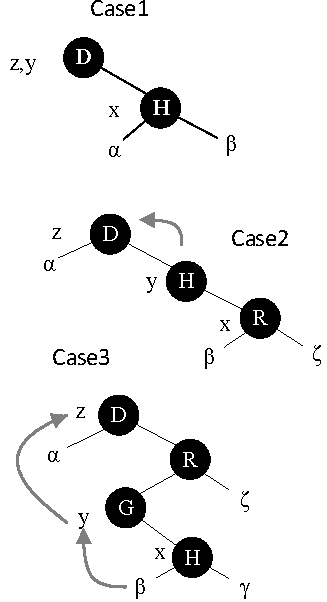
\includegraphics[width=\textwidth]{rb_delete_cases_single.pdf}
  \caption{default}
  \label{fig:figure2}
  \end{minipage}
  \end{figure}
  This is where the table goes with text wrapping around it. You may 
embed tabular environment inside wraptable environment and customize as you like.

Most gulls, particularly Larus species, are ground nesting carnivores,
which will take live food or scavenge opportunistically. The live food
often includes crabs and small fish. Apart from the kittiwakes, gulls
are typically coastal or inland species, rarely venturing far out to sea.
The large species take up to four years to attain full adult plumage,
but two years is typical for small gulls.
\end{document}